%%%% Better Poster for
%%%% The Collapse of Heterogeneity in Silicon Philosophers
%%%% Yuanming Shi and Andreas Haupt
%%%%
%%%% Layout: Rafael Bailo's betterposter class
%%%% Design: Mike Morrison

\documentclass[a0paper,fleqn]{betterposter}

\usepackage{booktabs}
\usepackage{array}

%% Side columns wide enough for compact paper tables.
\setlength{\leftbarwidth}{0.24\paperwidth}
\setlength{\rightbarwidth}{0.33\paperwidth}

\renewcommand{\section}[1]{%
\vspace{0.55em}{\fontsizesection\selectfont
\textbf{\leavevmode #1}}\\[0.2em]
}

\renewcommand{\fontsizemain}{\fontsize{48}{58}\selectfont}
\renewcommand{\fontsizetitle}{\fontsize{42}{50}\selectfont}
\renewcommand{\fontsizeauthor}{\fontsize{24}{32}\selectfont}
\renewcommand{\fontsizesection}{\fontsize{28}{36}\selectfont}
\renewcommand{\fontsizestandard}{\fontsize{22}{28}\selectfont}

\renewcommand{\maincolumnbackgroundcolor}{empirical}

\newcommand{\tablefont}{\fontsize{18}{24}\selectfont}
\newcommand{\tablenote}{\color{gray}\fontsize{16}{20}\selectfont}

\begin{document}
\betterposter{
%%%%%%%% MAIN COLUMN
\maincolumn{
A social world model is
adequate only if it matches
the \textbf{distribution of
human minds}.

\vspace{0.35em}
{\fontsize{38}{48}\selectfont
Silicon philosophers
\textbf{fail this test}:
they are \textbf{1.4--2.4$\times$}
too uniform, and they
disagree along the
\textbf{wrong axes}.
}
}{
\qrcode{img/qrcode}{img/smartphoneWhite}{
\textbf{Take a picture}
\\for the paper and
\\data explorer.
}
}

}{
%%%%%%%% LEFT COLUMN

\title{The Collapse of Heterogeneity\\in Silicon Philosophers}
\author{Yuanming Shi\quad Andreas Haupt}
\institution{Adobe Inc.\quad Stanford University}

\section{Question}
Can an LLM stand in for a
population of minds?

\section{Setup}
\begin{itemize}
\item 277 PhilPeople philosophers
\item 100 PhilPapers 2020 questions
\item 7 profile-conditioned LLMs
\item Temperature 0; Accept $\to$ Reject
coded onto $[0,1]$
\item Checked against PhilPapers 2020
($N=1{,}785$)
\end{itemize}

\section{Silicon sampling}
\begin{center}
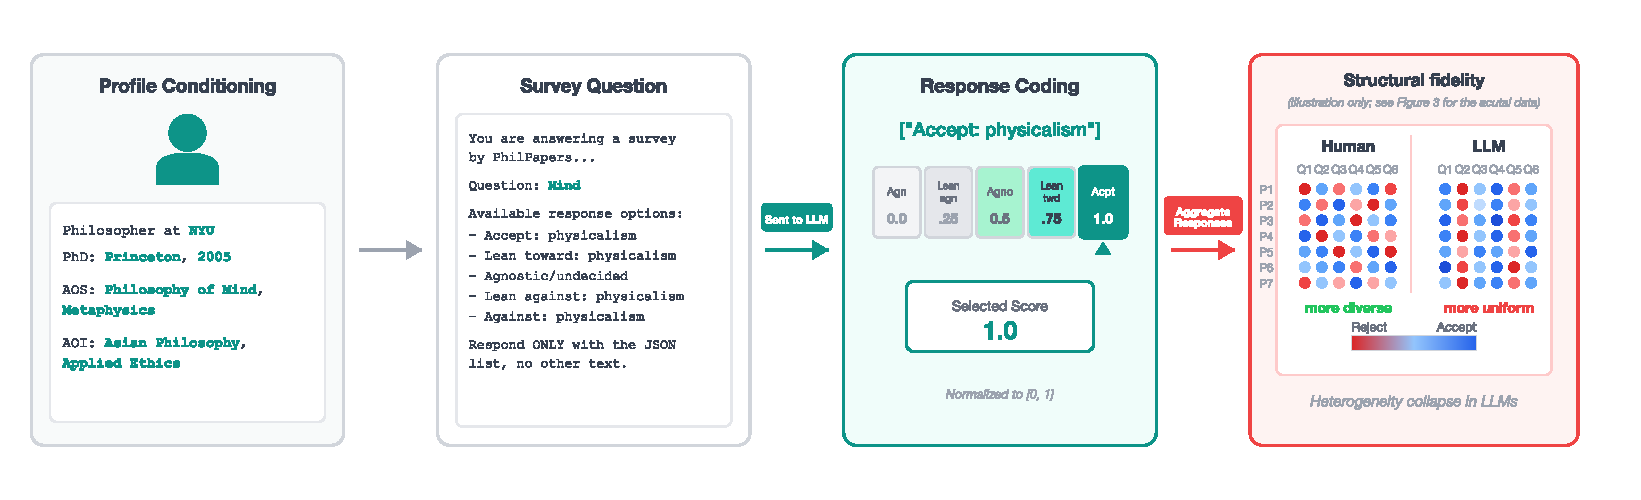
\includegraphics[width=\textwidth]{figures/silicon_sampling_pipeline}
\end{center}
{\tablenote Fig.~1. Profile $\to$ question $\to$ coded stance $\to$ fidelity.}

\section{Spread collapses (Table~1)}
{\tablefont
\begin{tabular}{@{}l r r@{}}
\toprule
Source & Resp\% & Per-Q Var \\
\midrule
Human & 19.1 & 0.062 \\
Claude Sonnet 4.5 & 36.2 & 0.043 \\
Llama 3.1 8B & 63.0 & 0.042 \\
Mistral 7B & 70.0 & 0.029 \\
GPT-4o & 48.4 & 0.027 \\
GPT-5.1 & 49.1 & 0.026 \\
\bottomrule
\end{tabular}\\[0.3em]
}
{\tablenote Humans are $1.4$--$2.4\times$ more variable than every LLM.}

\section{Correlations inflate (Table~2)}
{\tablefont
\begin{tabular}{@{}l r r@{}}
\toprule
Source & Max $|r|$ & \% Sig. \\
\midrule
PhilPapers 2020 & 0.29 & ${\sim}$5 \\
Human sample & 0.57 & ${\sim}$5 \\
Claude Sonnet 4.5 & 0.82 & 13.7 \\
GPT-5.1 & 0.93 & 13.3 \\
\bottomrule
\end{tabular}\\[0.3em]
}
{\tablenote LLMs invent 2--3$\times$ more significant specialist links.}

\vfill
{\color{gray}\fontsize{18}{22}\selectfont
ACM FAccT 2026
}

}{
%%%%%%%% RIGHT COLUMN

\section{Human vs.\ Claude}
\begin{center}
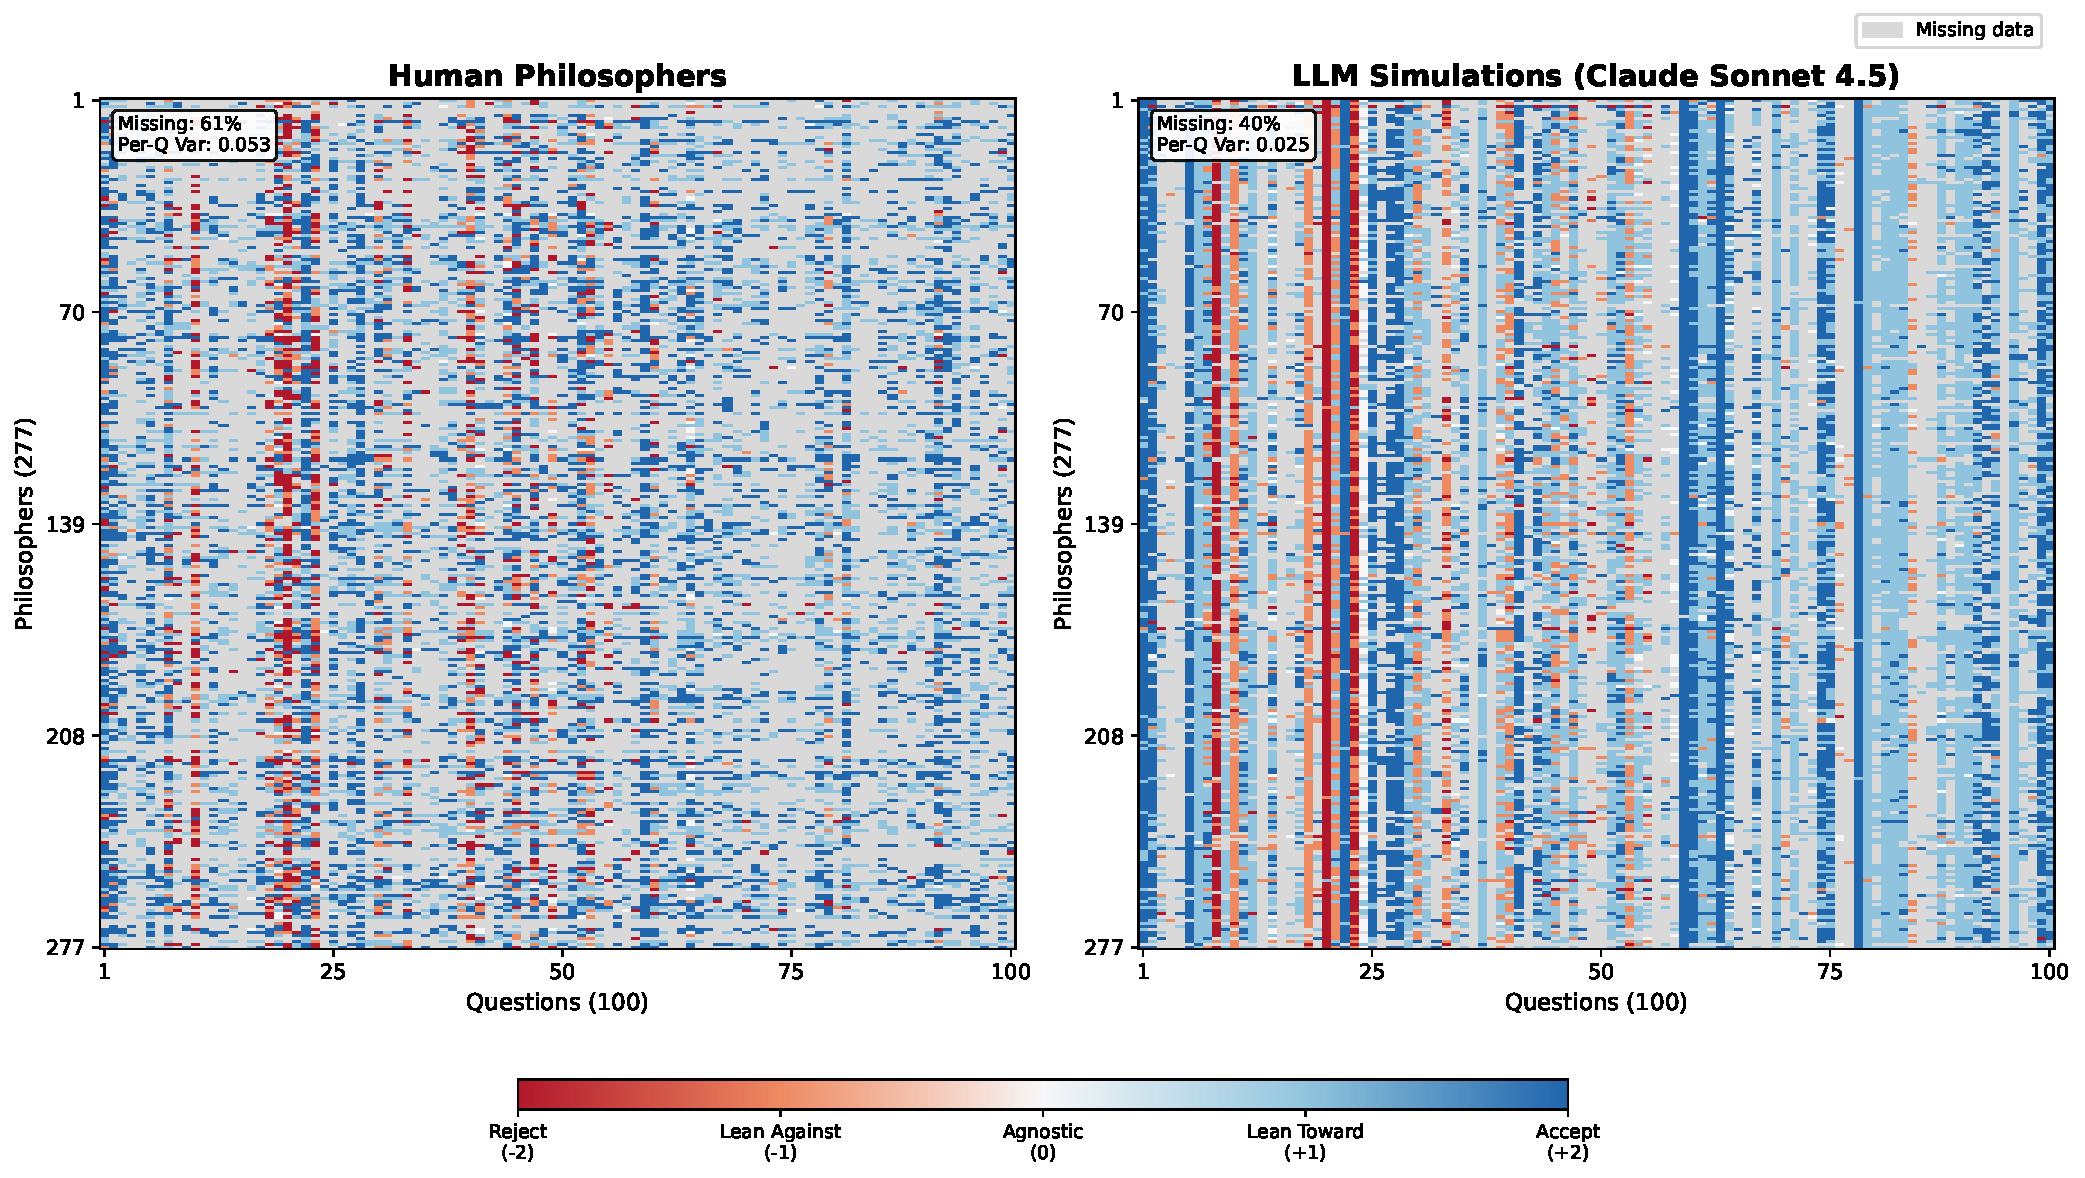
\includegraphics[width=\textwidth]{figures/figure1_human_vs_sonnet}
\end{center}
{\tablenote Fig.~3a. Each cell is one philosopher on one question.
Humans speckled; Claude forms vertical bands.}

\section{Wrong axes (Table~7)}
{\tablefont
\begin{tabular}{@{}l r r@{}}
\toprule
Source & Var(6) & Elem $r$ \\
\midrule
Human & 22.4\% & --- \\
Claude Sonnet 4.5 & 31.7\% & 0.108 \\
Llama 3.1 8B (FT) & 33.5\% & 0.079 \\
GPT-4o & 28.0\% & 0.055 \\
GPT-5.1 & 28.9\% & 0.049 \\
\bottomrule
\end{tabular}\\[0.3em]
}
{\tablenote Models collapse disagreement onto fewer, topical axes.
Best pairwise alignment is still weak ($r\le 0.11$).}

\section{Stereotypes fill the gap (Table~3)}
{\tablefont
\begin{tabular}{@{}p{0.55\textwidth} r r@{}}
\toprule
Specialist effect & Human & LLM \\
\midrule
Biology $\to$ biol.\ identity & $+11$\,pp & $+43$\,pp \\
Biology $\to$ psych.\ identity & $+4$\,pp & $-66$\,pp \\
Ancient $\to$ Aristotelian & $+2$\,pp & $+69$\,pp \\
\bottomrule
\end{tabular}\\[0.3em]
}
{\tablenote Ground truth n.s.; LLM effects significant in 3--7 of 7 models.}

\section{DPO does not restore it (Table~10)}
{\tablefont
\begin{tabular}{@{}l r r@{}}
\toprule
Llama 3.1 8B & Entropy & Corr.\ KL \\
\midrule
Base & 0.662 & 0.155 \\
DPO fine-tuned & 0.605 & 0.062 \\
\bottomrule
\end{tabular}\\[0.3em]
}
{\tablenote Structure improves (KL $-60\%$); diversity falls (entropy $-8.6\%$).}

}
\end{document}
